\documentclass[a4paper,12pt]{article}
\usepackage[margin=2cm,top=1cm]{geometry}		
\usepackage[thinfonts]{uglix2}
\begin{document}
{\large\bfseries \scshape Nom Prénom : \makebox[6cm]{\dotfill}}\\

\textbf{Question 1}\\

\carreauxseyes{16.8}{9.6}\\


\textbf{Question 2}\\

\carreauxseyes{16.8}{9.6}\\

\newpage

\textbf{Question 3}\\

\carreauxseyes{16.8}{6.4}\\

\textbf{Question 4}
\begin{pseudocode}\begin{minted}{pseudocode}
fonction compresse(ligne)

    variables
        résultat : liste
        valeur, compteur, i : entiers
        
    résultat ← liste vide
    valeur ← 0              # on part de la valeur 0
    compteur ← 0            # au départ il y en a zéro
    i ← 0                   # on commence au début de la ligne
    tant que i < longueur(ligne)
    
        si ligne[i] = .........
        
            compteur ← compteur + 1
        sinon
            valeur ← 1 - valeur
            ajouter compteur à la fin de résultat
            compteur ← 1
            
        ..........
        
    ajouter compteur à la fin de résultat
    renvoyer résultat
\end{minted}
\end{pseudocode}

\textbf{Question 5}

\begin{center}
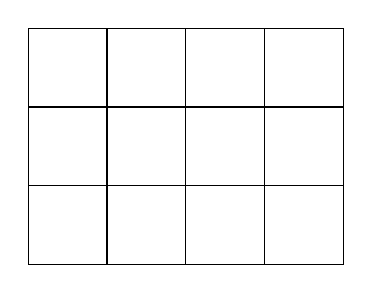
\begin{tikzpicture}
\draw (0,2) rectangle (1,3);
\draw (1,2) rectangle (2,3);
\draw (2,2) rectangle (3,3);
\draw (3,2) rectangle (4,3);
\draw (0,1) rectangle (1,2);
\draw (1,1) rectangle (2,2);
\draw (2,1) rectangle (3,2);
\draw (3,1) rectangle (4,2);
\draw (0,0) rectangle (1,1);
\draw (1,0) rectangle (2,1);
\draw (2,0) rectangle (3,1);
\draw (3,0) rectangle (4,1);
\end{tikzpicture}
\end{center}

\end{document}
